\pagebreak
\subsection{Task 4: Configuring and Testing Group Policy}
Using the `Group Policy Management' tool, create new group policies (taking care to use sensible names) under the relevant Organisation Unit and then edit them to add the specific policies that are to be applied to that OU.

\begin{enumerate}[series=task4methodology1]
  \item Create a group policy to set up Folder Redirection for all users: `Users' and `SysOps'. This is done with the following process:
    \begin{enumerate}[label=(\alph*)]
      \item Create a new Group Policy Object for all users by right-click `Resources' and selecting `Create a GPO in this domain, and Link it here'. Set the name of the new GPO to `FolderRedirection'.
        \begin{figure}[H]
          \centering
          \captionsetup{skip=2pt}
          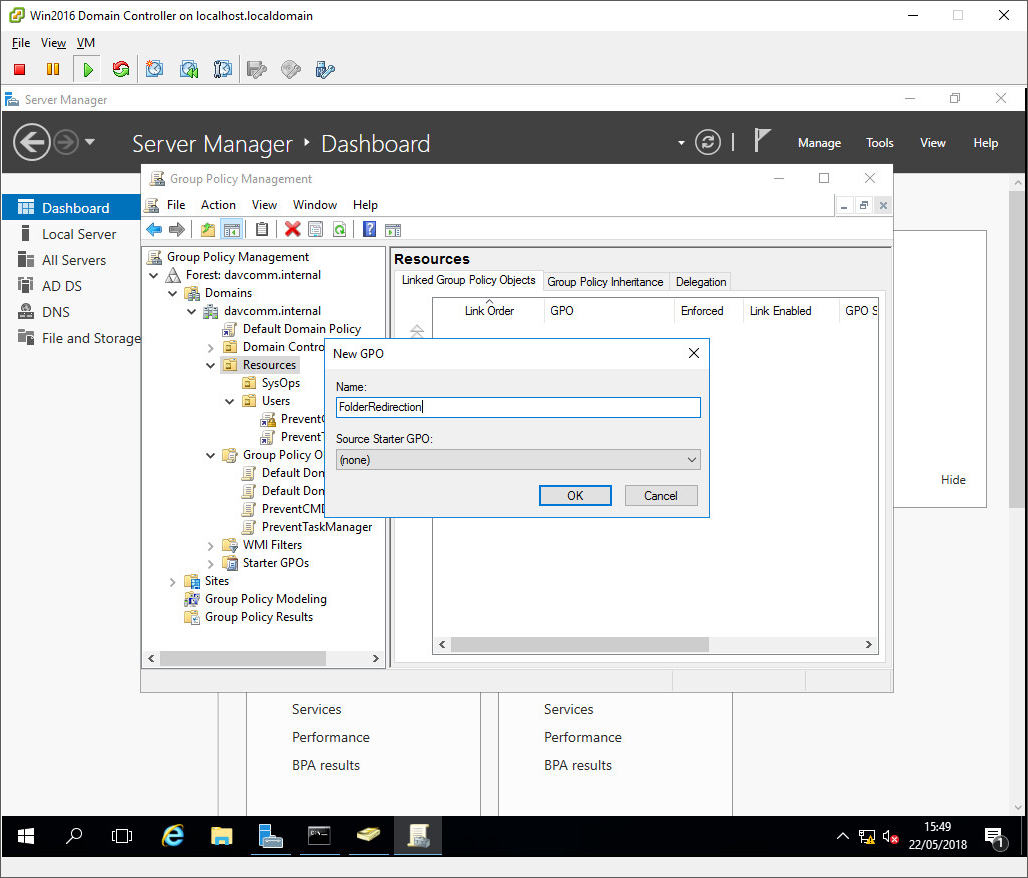
\includegraphics[width=\textwidth]{task4_01_gp_03_set_01}
          \caption{[4] Server 2016 DC: Naming a new GPO}
          \label{fig:task4:gp3a1}
        \end{figure}
      \item Right-click the newly created GPO and select `Edit'. Navigate to `User Configuration > Policies > Windows Settings > Folder Redirection'.
        \begin{figure}[H]
          \centering
          \captionsetup{skip=2pt}
          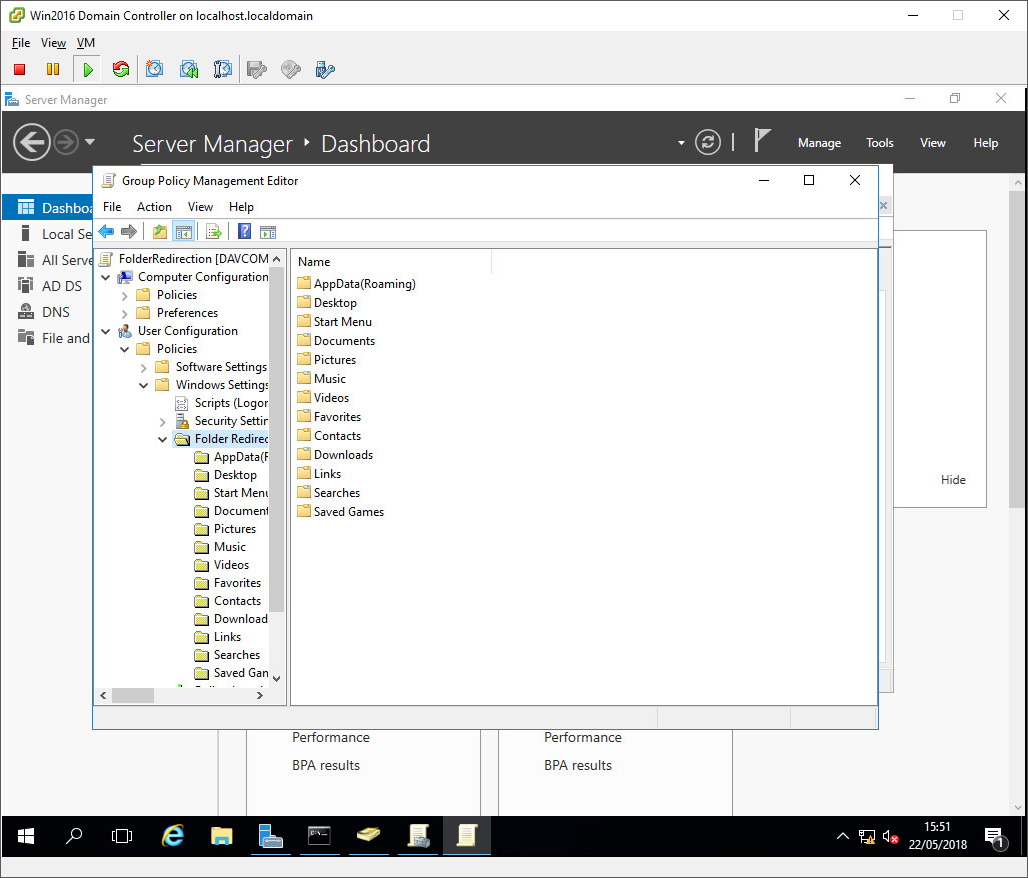
\includegraphics[width=\textwidth]{task4_01_gp_03_set_03}
          \caption{[4] Server 2016 DC: Applying a folder redirection policy}
          \label{fig:task4:gp3a3}
        \end{figure}
      \item Right-click on the folder that is to be redirected and select `Properties'. For this demonstration, I only redirected `Documents' but this process could be repeated to redirect as many folders as desired. Under `Target' in the `Documents Properties', set the setting to `Basic' in order to redirect everyone's folders to the same location and set the `Root Path' to the path of the `usershare` on the User Server. Once this is done click OK.
        \begin{figure}[H]
          \centering
          \captionsetup{skip=2pt}
          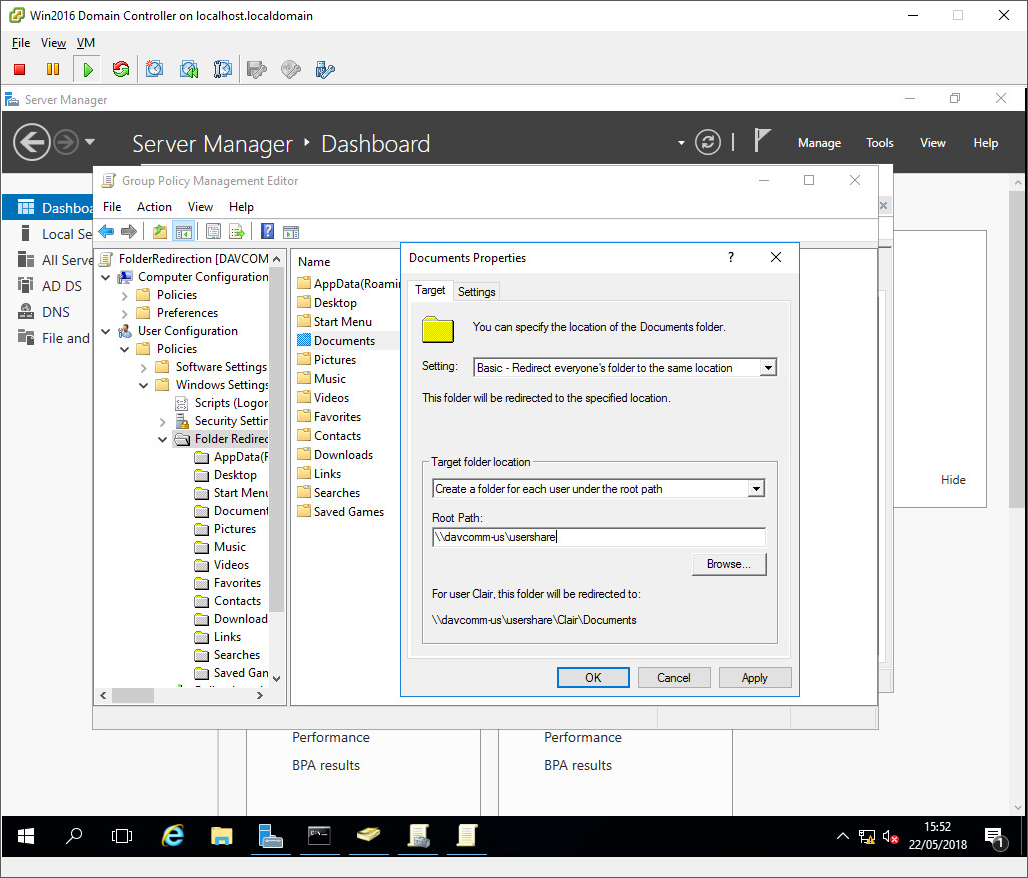
\includegraphics[width=\textwidth]{task4_01_gp_03_set_04}
          \caption{[4] Server 2016 DC: Configuring the folder redirection GPO}
          \label{fig:task4:gp3a4}
        \end{figure}
      \item Once this is done, check that the policy has been applied correctly to the users on the client by logging into a user and verifying that the `Documents' folder has been redirected.
        \begin{figure}[H]
          \centering
          \captionsetup{skip=2pt}
          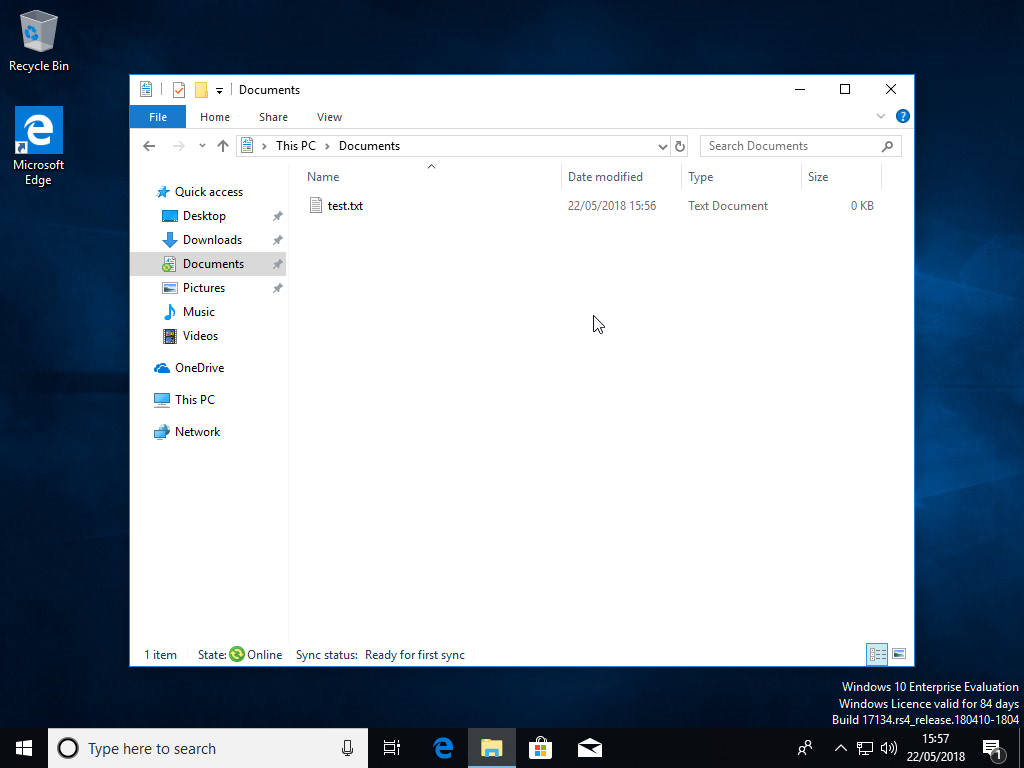
\includegraphics[width=\textwidth]{IY1D403_Windows_10_x64_Client-2018-05-22-15-57-16}
          \caption{[4] Win 10 Client: Verifying the Folder Redirection GPO works}
          \label{fig:task4:gp3b1}
        \end{figure}
      \item Finally, verify that the security configuration for the share works correctly by attempting to access a different users redirected folders. In the figure below, it can be seen that the other users' folders are not shown to the user that is logged in. It is also not possible to access other users' folders by explicitly attempting to navigate to their folder by the path name.
        \begin{figure}[H]
          \centering
          \captionsetup{skip=2pt}
          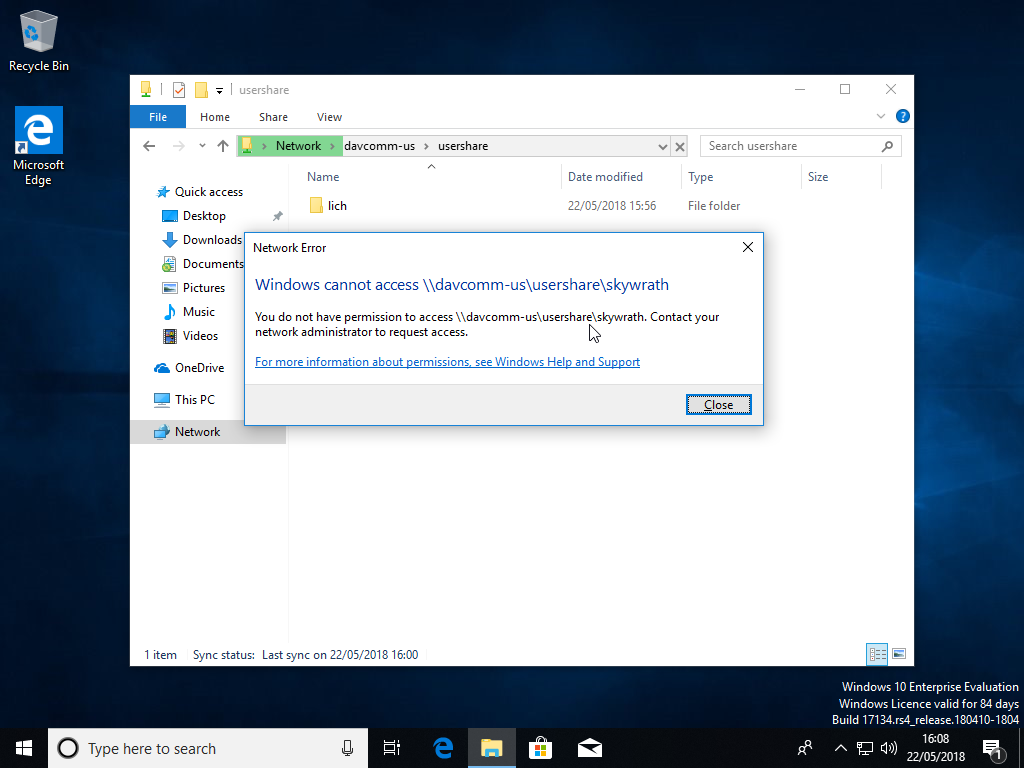
\includegraphics[width=\textwidth]{IY1D403_Windows_10_x64_Client-2018-05-22-16-08-20}
          \caption{[4] Win 10 Client: Verifying the Folder Redirection GPO security configuration}
          \label{fig:task4:gp3b2}
        \end{figure}
    \end{enumerate}
  \item Create a group policy to `Prevent access to the command prompt' for members of the `Users' OU and then check that it works by logging in as one of the users on the client.
    \begin{figure}[H]
      \centering
      \captionsetup{skip=2pt}
      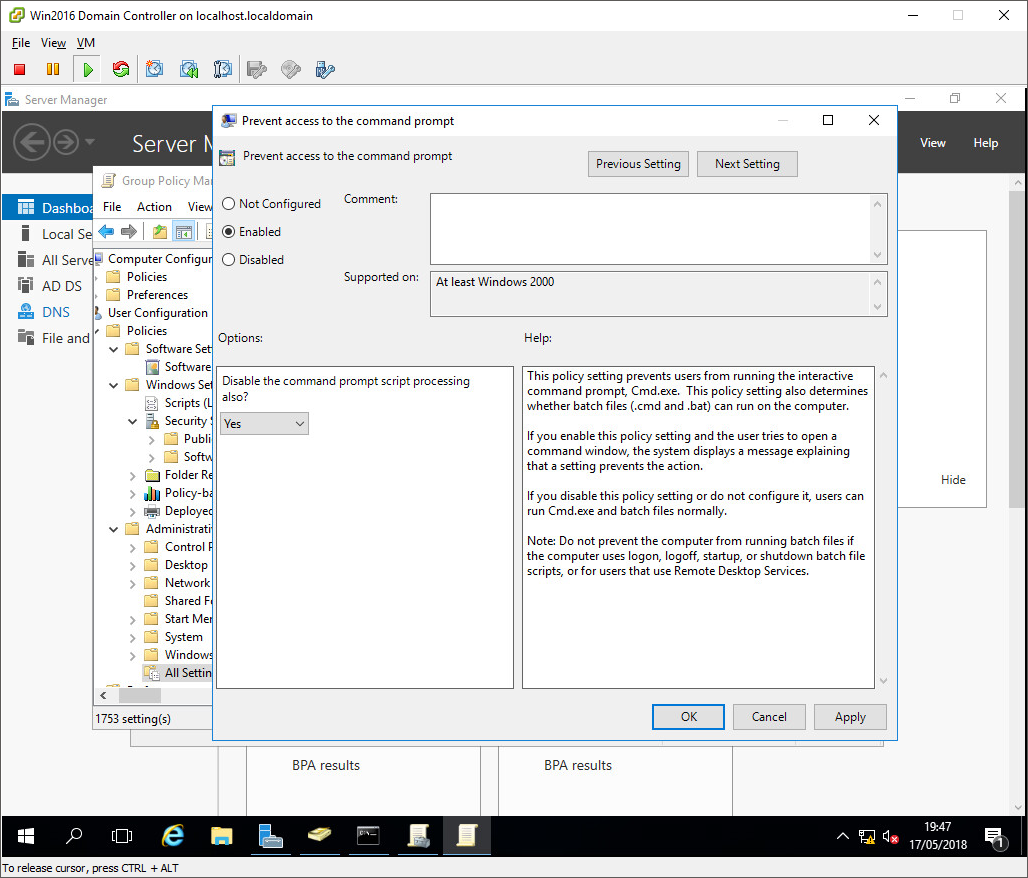
\includegraphics[width=\textwidth]{task4_01_gp_01_set_01}
      \caption{[4] Server 2016 DC: Creating a GPO to disable the Command Prompt}
      \label{fig:task4:gp1a}
    \end{figure}
    \begin{figure}[H]
      \centering
      \captionsetup{skip=2pt}
      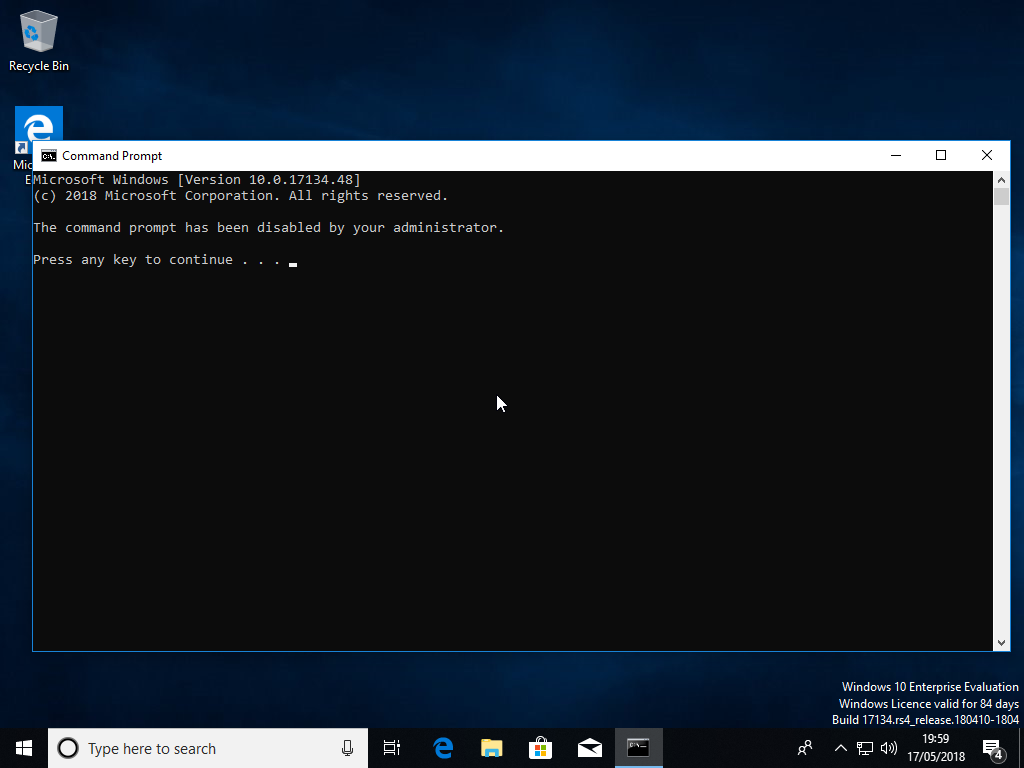
\includegraphics[width=\textwidth]{IY1D403_Windows_10_x64_Client-2018-05-17-20-00-05}
      \caption{[4] Win 10 Client: Checking the GPO to disable Command Prompt}
      \label{fig:task4:gp1b}
    \end{figure}
  \item Create a group policy to `Remove Task Manager' for members of the `Users' OU and then check that it works by logging in as one of the users on the client.
    \begin{figure}[H]
      \centering
      \captionsetup{skip=2pt}
      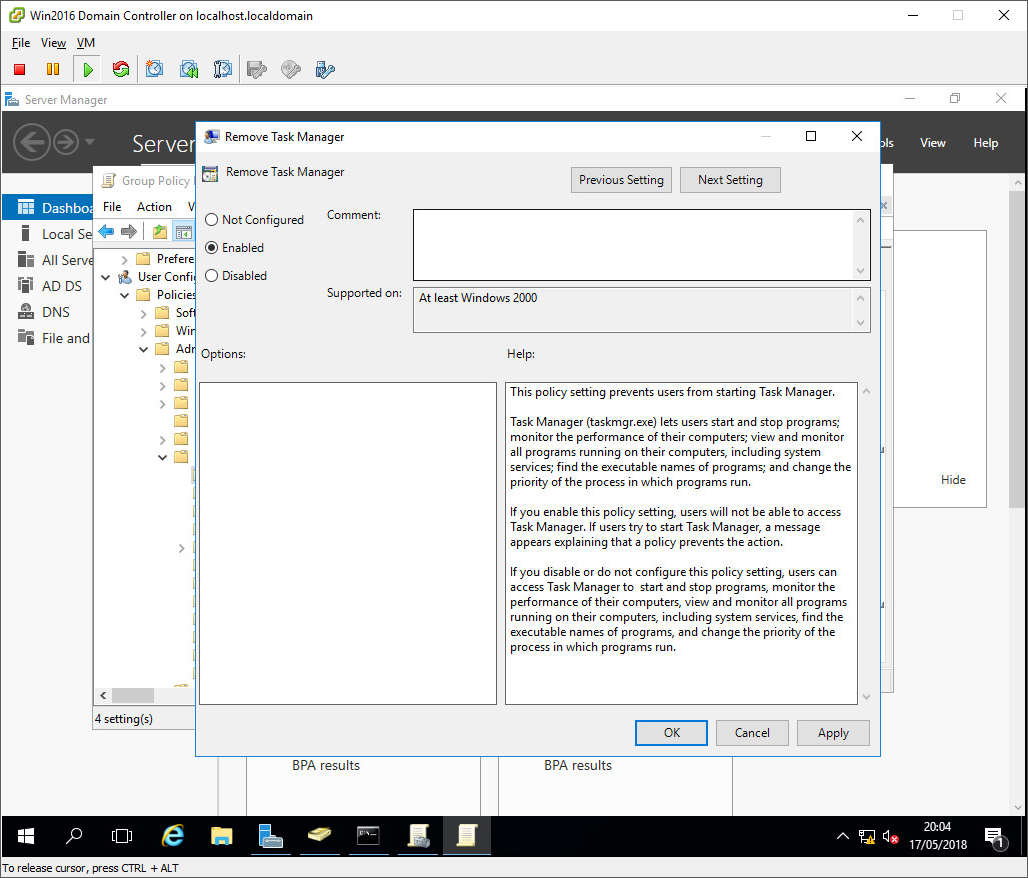
\includegraphics[width=\textwidth]{task4_01_gp_02_set_01}
      \caption{[4] Server 2016 DC: Creating a GPO to disable Task Manager}
      \label{fig:task4:gp2a}
    \end{figure}
    \begin{figure}[H]
      \centering
      \captionsetup{skip=2pt}
      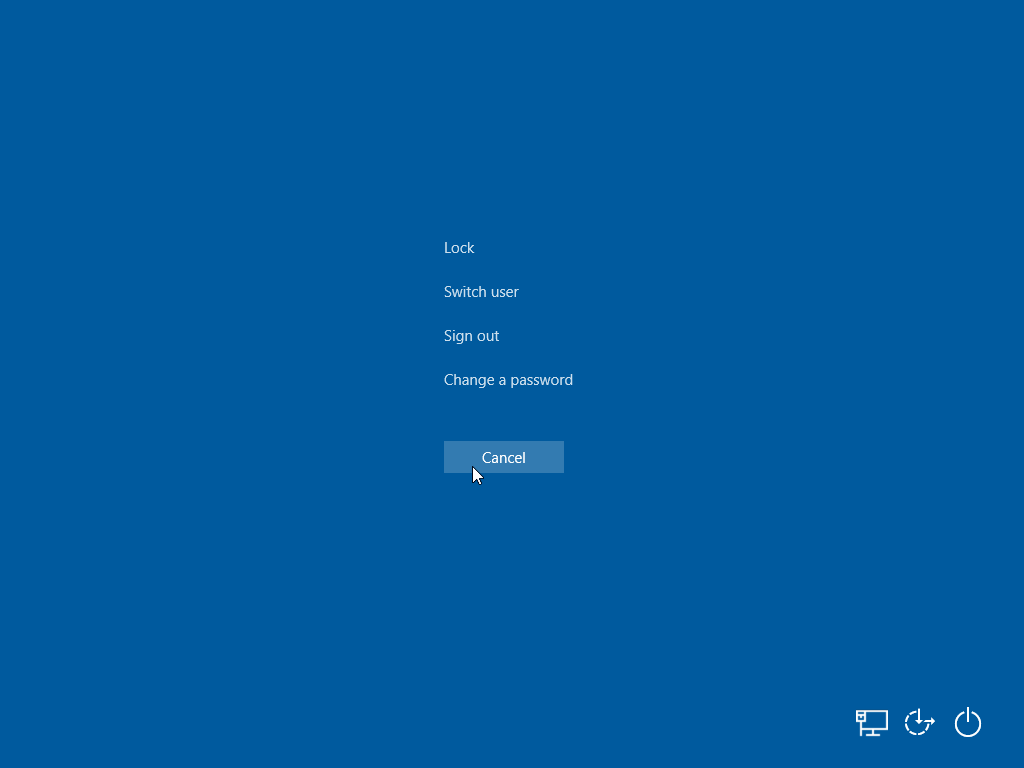
\includegraphics[width=\textwidth]{IY1D403_Windows_10_x64_Client-2018-05-17-20-06-07}
      \caption{[4] Win 10 Client: Checking the GPO to disable Task Manager}
      \label{fig:task4:gp2b}
    \end{figure}
\end{enumerate}
